%!TEX root = ../thesis.tex
\begin{savequote}[75mm]
Nulla facilisi. In vel sem. Morbi id urna in diam dignissim feugiat. Proin molestie tortor eu velit. Aliquam erat volutpat. Nullam ultrices, diam tempus vulputate egestas, eros pede varius leo.
\qauthor{Quoteauthor Lastname}
\end{savequote}

\chapter{Projet implementation}

This chapter is the core of this document and describes the way that this project has been implemented according to the work plan described in Chapter 2.

It is structured in four main sections, each representing a period:
\begin{enumerate}
	\item Learning stage
	\item Implementation
	\item Testing
	\item Feedback
\end{enumerate}

%todo rivedere tutto
\section{Learning stage - CAMBIARE NOME}

	This phase corresponds to the first two weeks of the internship.
	As described in the work plan in this first period the main task was to understand what the tools are.
	At first I have started to search information about Jira and Confluence on Google.
	%todo aggiungere riferimento a official documentation
	The first tools I have started researching was Jira, and the official documentation is very well organized.
	\begin{figure}[H]
		\centering
		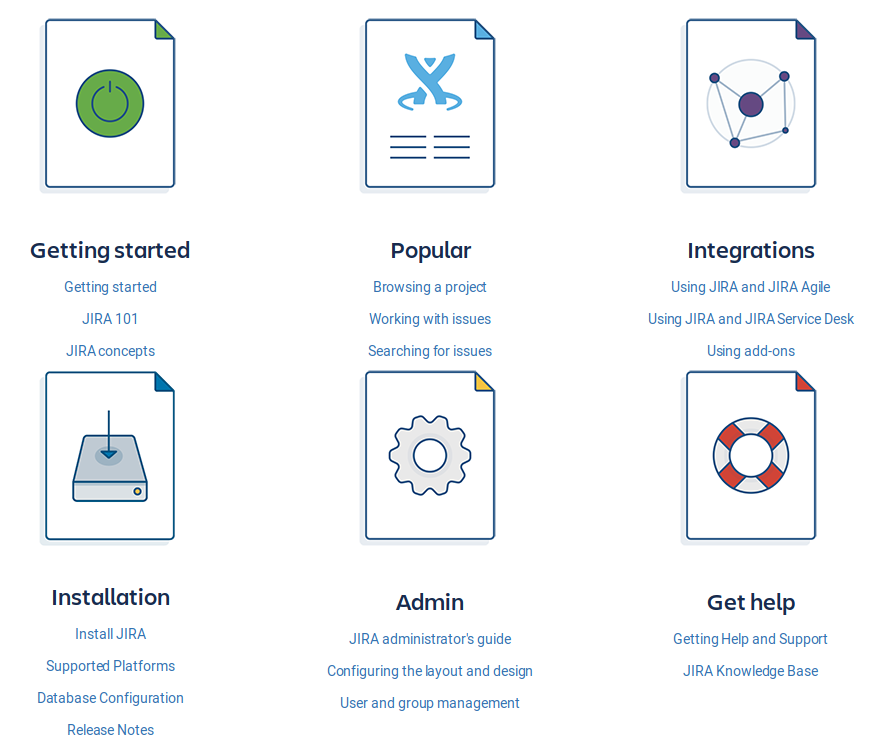
\includegraphics[width=1\textwidth]{resources/jira_documentation}\\
		\caption{Screenshot of the Jira Documentation homepage from the Atlassian Support website}
	\end{figure}
	
	This documentation is very easy to navigate because it versioned for each release, major and minor, of the software, plus it contains links to related pages.
	
	If there is a reference about a Confluence webpage, this is added as a link.
	Vice versa on the Confluence documentation, if there is a Jira reference, it links to the latter's documentation.
	
	Both Jira and Confluence have a bug reporting and issue tracking section in their documentation.
	\begin{figure}[H]
		\centering
		\includegraphics[width=1\textwidth]{resources/confluence_documentation_issues}\\
		\caption{The issues related with Jira and Confluence are handled by a dedicated Jira Cloud instance}
	\end{figure}
	
	If a webpage in the documentation is related to an issue, the latter is showed at the end of the page with its status and a link to its dedicated section.
	
	%todo rivedere userbase
	The Confluence and Jira documentation are both written and hosted using Confluence, showing how powerful can be this tool for handling a wiki for such a complex software that has a large userbase.
	
	Confluence documentation is structured like Jira's, very easy to access and consult.
	
	Another bonus is that it is public and free to consult, despite the software is not.
	This may seem like an obvious choice but not all vendors do it: RedHat for example let's you consult their documentation only if you log into the website.
	
\section{Initial installation and configuration}
	
	Study of the documentation and installation on the meantime, learn by doing
	
	\subsection{Work tools and installation}
		
		Linux workstation and CentOS VM with 512GB of storage and 32GB of RAM
	
		installazione dei software\\
		
		As refered to 
		
		ho lavorato su una vm centos con queste caratteristiche ...
		
	\subsection{Additional software}
		POSTGRES\\
		mi ha fatto ritardare rispetto al piano di lavoro? no, mi ero aspettato ci fossero software terzi da configurare / imparare
	
	\subsection{First configuration}
		interconnessione tra i tool
	
	\subsection{Understanding the products}
		creazione di progetti di mock\\
		interconnetterli\\
		capire il workflow delle issue\\
		utilizzare gitlab (con account personale su server aziendale e progettini di mock) per effettuare transizioni automatiche delle issue (spiegare correlazione tra progetti in gitlab e in jira)

	\subsection{Requirements change}
		non usare bitbucket ma gitlab\\
		visto il grosso ammontare di elementi customizzabili è stato necessario scremare le cose e capire cosa si poteva facilmente aggiungere e cosa lasciare per dopo\\
		abbellimento dell'environment
		
		%todo logo dei due prodotti

	\subsection{Customizing the user interface}
		a causa della poca disponibilità in questo primo periodo di marco e paolo che utilizzeranno questo tool in maniera intensiva rispetto al tutor, ho fatto un task secondario come quello della personalizzazione dell'interfaccia grafica
	
		%todo immagini interfaccia grafica prima e dopo
	
	\subsection{snapshot della macchina per salvare il lavoro svolto per ora}
		parlare di milestone / baseline\\
		come le ho pensate nel piano di lavoro

\section{First realistic mock projects and feedback}

	This phase corresponds to ... in the work plan

	\subsection{The projects}
		idee del tutor\\
		prime demo con lui per capire se questo tool effettivamente copre le necessità di base dell'azienda
		
	\subsection{Integrating with GitLab}
		in questo periodo vista la scarista di opzioni di gitla nativo si è scelto di usare un plugin\\
		(decontestualizzare il tempo, a posteriori, ragionando per milestone)\\
		visto integrazione nativa\\
		scelta di utilizzare un plugin\\
		costa ma è migliore (descrivere da quale punto di vista)
	
	\subsection{First meetings to present the progress}
		primo feedback e discussioni di come può evolvere il progetto e come può essere applicato ai loro workflow\\
		riflessioni personali: a questo punto sto rispettando il piano di lavoro iniziale? sono in ritardo / anticipo?
	
	\subsection{New requirements change}
		giustificare --> dopo fase di studio / riscontro\\
		cosa può essere implementato subito, cosa no, come viene usato\\
		campi e workflow custom\\
		mapping tra processi jira e interni (sprint)
	
	\subsection{Documentation}
		scrittura della bozza di documentazione e passaggio della documentazione in confluence
		
	\subsection{New snapshot of the machine}
		nuova baseline / milestone

\section{Transitioning to production}

	This phase corresponds to ... in the work plan

	After the approval for using the tools by other departments (R\&D) it's time to transition it / move it to production
	
	\subsection{Migrating data from Redmine}
		tool automatico di migrazione
		collegamento con redmine, lo fa in maniera automatica
		e se va male? c'è sempre lo snapshot
	
	\subsection{First non mock projects}
	
	\subsection{Fine tuning of the final product}
		interazione con le persone
		in base alle necessità degli utenti e di come lo usano faccio minime modifiche in produzione
		miglioramento della documentazione
	
	\subsection{How are these tools being used}
		è veramente agile? 
		è un dialetto?
		è un misto?
		perchè athonet lo sta usando in questo modo?

\section{Final feedback and what else could be implemented in the future}

	This phase corresponds to ... in the work plan

	\subsection{Final feedback from the users}
		feedback da parte del tutor
		
		feedback da responsabile strategia aziendale (gl)
		feedback da responsabile del prodotto (aka product ownner / hesham)
		feedback da responsabile sviluppo + testing
			
		feedback da parte di tutti gli utenti
	
	\subsection{What Athonet plans to do with these new tools}
		arrivare ad utilizzare agile in maniera rigida?
		continuare a fare misto?
